\subsection{Perceptual loss}
\label{appendix:perceptual_loss}

Perceptual loss evaluates the disparity between the high-level features of two images (usually in the context of generative models, we compare one generated image and one from the dataset). These features are usually obtained using pre-trained convolutional neural networks (CNNs), typically VGG type network (VGG16, VGG-Net).

An example of when perceptual loss becomes useful is when we measure difference between two images using MSE. If we take the same image, move it 1 pixel to the left, and calculate the MSE between the two images, the MSE will be very high, even though the images are almost identical. Perceptual loss, on the other hand, will be able to tell that the images are almost identical, because the high-level features of the images are the same. This property is useful in generative models, where we want to generate images that are similar to the images in the dataset, as well as other tasks.

\begin{figure}
    \centering
    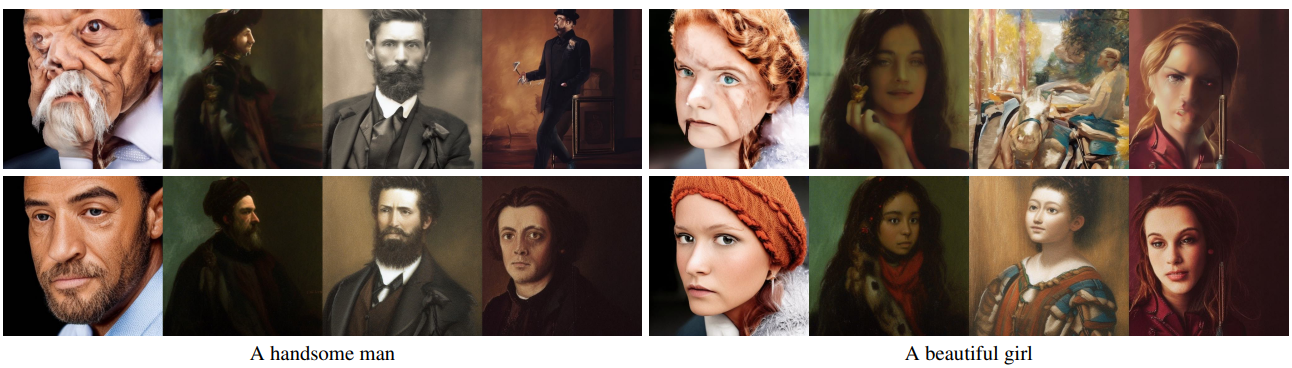
\includegraphics[width=1\textwidth]{images/appendix/perceptual_loss.png}
    \caption{Diffusion models trained with mean squared error loss (top row) generate unrealistic samples without classifier-free guidance. A proposed self-perceptual loss fixes this issue and can generate realistic samples without classifier-free guidance \cite{perceptual_loss_in_diffusion}.}
\end{figure}

\textbf{Methodology.} The perceptual loss is calculated by passing the images through a pre-trained CNN (usually VGG, see appendix \ref{appendix:vgg_network}), and extracting the high-level features from the network (the feature maps in the middle layers) through various layers of this network. The high-level features are then compared using a loss function, such as MSE or L1 loss, rather than the pixels themselves. 



\begin{lstlisting}[language=Python, caption={Example of perceptual loss implementation. Typically we don't compare the lower layers, since they contain pixel level features, and not semantics.}]
def perceptual_loss(generated_img, target_img, feature_extractor, layers):
    loss = 0
    for layer in layers:
        generated_features = feature_extractor(generated_img, layer)
        target_features = feature_extractor(target_img, layer)
        loss += torch.mean((generated_features - target_features) ** 2)
    return loss
\end{lstlisting}
